\documentclass[a4paper,12pt]{article}

\usepackage[utf8]{inputenc}
\usepackage[T1]{fontenc}
\usepackage[a4paper,total={150mm,240mm}]{geometry}
\usepackage{amsmath}
\usepackage{amsfonts}
\usepackage{amsthm}
\usepackage{amscd}
\usepackage{grffile}
\usepackage{tikz} 
\usetikzlibrary{patterns}
\usepackage{eurosym} 
\usepackage{graphicx}
\usepackage{color}
\usepackage{listings}
\lstset{language=C++, basicstyle=\ttfamily, 
  keywordstyle=\color{black}\bfseries, tabsize=4, stringstyle=\ttfamily,
  commentstyle=\itshape, extendedchars=true, escapeinside={/*@}{@*/}}
\usepackage{paralist}
\usepackage{curves}
\usepackage{calc}
\usepackage{picinpar}
\usepackage{enumerate}
\usepackage{algpseudocode}
\usepackage{bm}
\usepackage{multibib}
\usepackage{hyperref}
\usepackage{textcase}
\usepackage{nicefrac}

\definecolor{listingbg}{gray}{0.95}

\theoremstyle{definition}
\newtheorem{exm}{Example}

%\title{DUNE PDELab ---
%Mathematical Abstractions for the Numerical Solution of Partial Differential Equations}
%\author{Peter Bastian\\
%  Universität Heidelberg, \\
%  Interdisziplinäres Zentrum für Wissenschaftliches Rechnen\\
%  Im Neuenheimer Feld 368, D-69120 Heidelberg\\
%  \url{Peter.Bastian@iwr.uni-heidelberg.de}
%}
%\date{\today}
%
\begin{document}

\begin{center}
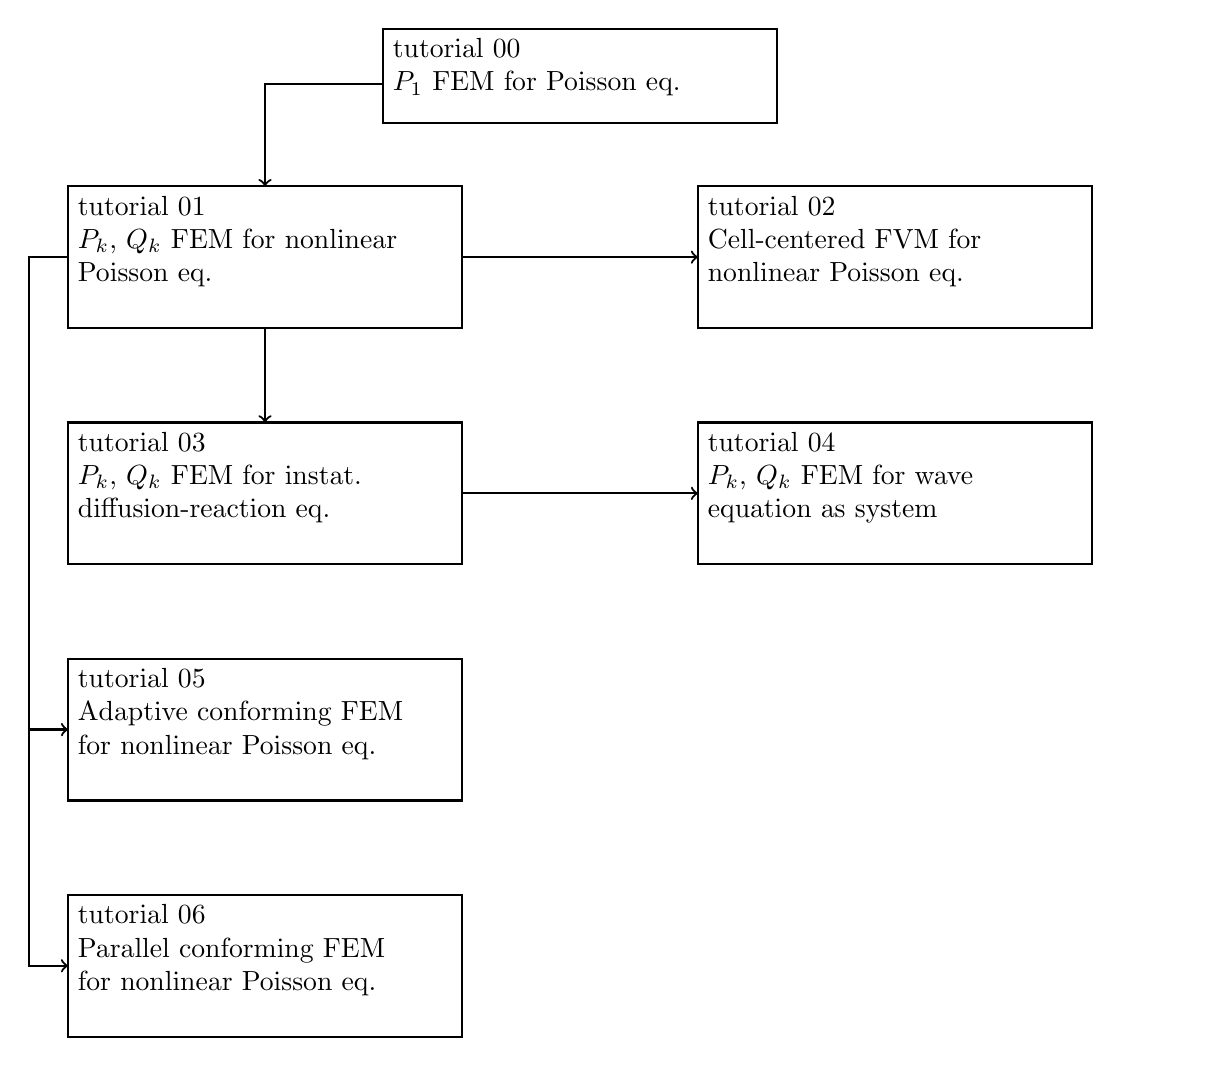
\begin{tikzpicture}[scale=1.0]
% tutorial 00
\draw[thick] (6,21)  rectangle (11,19.8);
\node[below right] at (6,21) {\begin{minipage}{6cm}
tutorial 00\\ 
$P_1$ FEM for Poisson eq.
\end{minipage}};
% tutorial 01
\draw[thick] (2,19)  rectangle (7,17.2);
\node[below right] at (2,19) {
\begin{minipage}{6cm}
tutorial 01\\ 
$P_k$, $Q_k$ FEM for nonlinear \\
Poisson eq.
\end{minipage}};
\draw[thick,->] (6,20.3) -- (4.5,20.3) -- (4.5,19);
% tutorial 02
\draw[thick] (10,19)  rectangle (15,17.2);
\node[below right] at (10,19) {
\begin{minipage}{6cm}
tutorial 02\\ 
Cell-centered FVM for \\
nonlinear Poisson eq.
\end{minipage}};
\draw[thick,->] (7,18.1) -- (10,18.1);
% tutorial 03
\draw[thick] (2,16)  rectangle (7,14.2);
\node[below right] at (2,16) {
\begin{minipage}{6cm}
tutorial 03\\ 
$P_k$, $Q_k$ FEM for instat.\\
diffusion-reaction eq.
\end{minipage}};
\draw[thick,->] (4.5,17.2) -- (4.5,16);
% tutorial 04
\draw[thick] (10,16)  rectangle (15,14.2);
\node[below right] at (10,16) {
\begin{minipage}{6cm}
tutorial 04\\ 
$P_k$, $Q_k$ FEM for wave\\
equation as system
\end{minipage}};
\draw[thick,->] (7,15.1) -- (10,15.1);
% tutorial 05
\draw[thick] (2,13)  rectangle (7,11.2);
\node[below right] at (2,13) {
\begin{minipage}{6cm}
tutorial 05\\ 
Adaptive conforming FEM\\
for nonlinear Poisson eq.
\end{minipage}};
\draw[thick,->] (2,18.1) -- (1.5,18.1) -- (1.5,12.1) -- (2,12.1);
% tutorial 06
\draw[thick] (2,10)  rectangle (7,8.2);
\node[below right] at (2,10) {
\begin{minipage}{6cm}
tutorial 06\\ 
Parallel conforming FEM\\
for nonlinear Poisson eq.
\end{minipage}};
\draw[thick,->] (1.5,12.1) -- (1.5,9.1) -- (2,9.1);
%\draw[draw=none,pattern=north east lines] (-0.25,0)  rectangle (0,3);
%\draw[very thick] (3,0) -- (3,3);
%\node at (1.5,2.2) {$T_{F'}^-, T_F^-$};
%\node at (4.5,2.2) {$T_F^+$};
%\draw[fill=black] (1.5,1.5)  circle (0.07);
%\node[below] at (1.5,1.5) {$x_{T_{F'}^-}, x_{T_F^-}$};
%\draw[fill=black] (4.5,1.5)  circle (0.07);
%\node[below] at (4.5,1.5) {$x_{T_F^+}$};
%\draw[thick,->] (3,1.5) -- (4,1.5);
%\draw[fill=black] (3,1.5)  circle (0.07);
%\node[left] at (3,1.5) {$x_{F}$};
%\node[below] at (3.5,1.5) {$\nu_F$};
%\node[left] at (3,0.5) {$F$};
%\draw[fill=black] (0,1.5)  circle (0.07);
%\draw[thick,->] (0,1.5) -- (-1,1.5);
%\node[right] at (0,1.5) {$x_{F'}$};
%\node[right] at (0,0.5) {$F'$};
\end{tikzpicture}
\end{center}


\end{document}
